\documentclass[10pt]{article}
\usepackage[a4paper,margin=2.0cm]{geometry}
\usepackage[T1]{fontenc}
\usepackage{lmodern}
\usepackage{microtype}
\usepackage{amsmath}
\usepackage{booktabs}
\usepackage{graphicx}
\usepackage{caption}
\usepackage{float}
\usepackage[hidelinks]{hyperref}
\graphicspath{{figures/}}
\setlength{\parskip}{0.45em}
\setlength{\parindent}{0pt}
\captionsetup{font=small,labelfont=bf}

\title{\vspace{-1.6em}On QMC stratification generating patterns with per-pixel alias tables\\ and how LeafAlias avoids that}
\author{}
\date{\vspace{-2.4em}}

\begin{document}
\maketitle
\vspace{-1.0em}

\textbf{The QMC argument is not a claim that LeafAlias exploits low-discrepancy input. It shows that per-pixel alias tables, despite their $O(1)$ sampling, have problems that make them unsuitable under certain conditions.}

\section*{1\quad How a per-pixel alias table turns a QMC point set into a pattern}

A per-pixel alias table~[1] maps a sample $(u,v)$ to bucket $k=\lfloor un\rfloor$ of $n$ (one per texel), keeps the bucket's own texel if $v<\tau_k$ and otherwise jumps to its alias; the leftovers of $u$ and $v$ place the sample inside the texel. With independent random numbers it has the same error as a 2D CDF; with a low-discrepancy sequence it does not. The $N$ values of $u$ that a pixel draws are spread almost evenly over $[0,1)$, so they visit the table at a nearly constant stride of $n/N$ buckets.

Vose's construction, as implemented in Falcor (\texttt{AliasTable.cpp}), lists below-mean and above-mean texels in scan order and pairs them in that order. Inside any region whose texels are all on the same side of the mean (a smooth sky, a dark hillside, a calm lake), consecutive buckets therefore own consecutive texels in scan order. In the emitter of Figure~\ref{fig:points} this holds for 96\% of consecutive bucket pairs. The constant stride through the table becomes a constant stride through the image: $n/N=WH/N$ texels, that is, $H/N$ rows, whatever the width. When $N$ divides $H$ (here $H=512$, $N=128$: exactly 4 rows), every sample of a pixel that falls in such a region lands in the same column. When $H/N$ is a simple fraction, they fall on a few columns or diagonals. Figure~\ref{fig:points} shows this for the first 500 Halton points: the 2D CDF keeps the even spread of the input, while per-pixel alias stacks the samples on the hillside into one column. In the spectrum (60000 points), the strongest spectral line is 41 times its median for per-pixel alias, against 1.4 for the 2D CDF and for BudgetLeafAlias.

\begin{figure}[H]
\centering
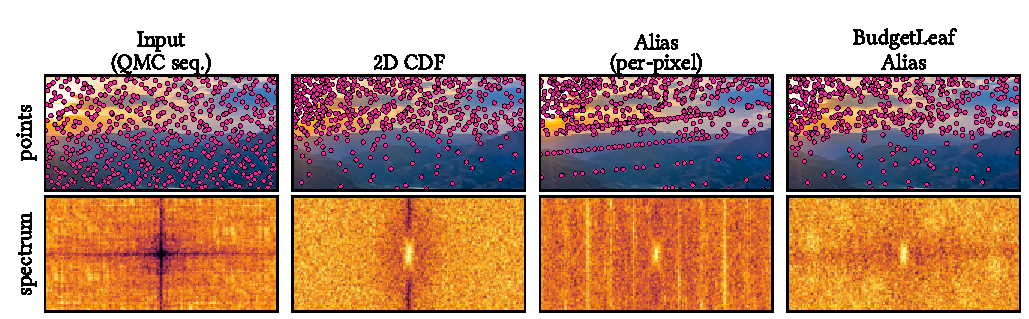
\includegraphics[width=\linewidth]{points_cinema_frame232_x704_y284_1024x507_500.pdf}
\caption{The paper's QMC comparison on a $1024\times512$ region of the Cinema texture (frame 232, $x=704$, $y=284$). Top: the first 500 points of the Halton sequence (bases 2, 3), as input and after each warp, over the whole region. Bottom: power spectrum of the first 60000 points. Per-pixel alias uses Falcor's table construction; BudgetLeafAlias uses the engine's 4000-leaf table.}
\label{fig:points}
\end{figure}

Two conditions must hold together. (i)~\emph{An aligned stride}: cropping the same region 5 texels narrower or shorter, the width does not matter (one column, 1.37$\times$ worse than pseudorandom), but at 507 rows the stride is 3.96 rows, the samples drift sideways and the error falls to 0.84$\times$. (ii)~\emph{Long scan-order runs}: a $512\times256$ sky region of the Rover texture is 2.0$\times$ worse than pseudorandom at 256 samples, but a $1024\times512$ window of more textured Rover content is not (0.96), because mixed bright and dark texels reorder the table. It does not depend on dynamic range. The textbook builder behind the submitted Figure~3 keeps scan order everywhere, hence its lattice; Falcor's builder does so only in uniform regions. Owen-scrambled sequences~[2] randomize the stride and, in our test, remove most of the effect.

\section*{2\quad What it costs in a rendering}

We render a diffuse floor lit by the textured area light through a fence (direct lighting, light sampling only, no MIS). Every pixel uses the Halton set with its own random toroidal shift, the standard per-pixel randomized QMC. The reference is exact (quadrature over the emitter, 0.3\% from a grid twice as fine). Figure~\ref{fig:scene} shows the setup; Figure~\ref{fig:fence} and Table~\ref{tab:fence} give the result for the region of Figure~\ref{fig:points} at 128 samples per pixel.

\begin{figure}[H]
\centering
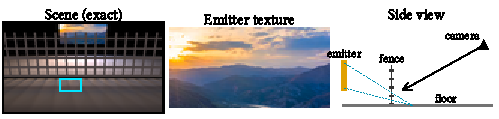
\includegraphics[width=0.92\linewidth]{scene_fence_cinema_frame232_x704_y284_1024x512_128spp.pdf}
\caption{The fence scene: exact render, emitter (the region of Figure~\ref{fig:points}), side view. Close-ups come from the cyan box.}
\label{fig:scene}
\end{figure}

\begin{figure}[H]
\centering
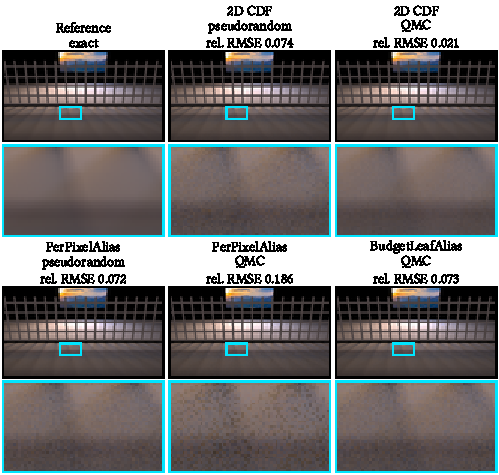
\includegraphics[width=0.88\linewidth]{fence_fence_cinema_frame232_x704_y284_1024x512_128spp.pdf}
\caption{Fence scene, 128 spp. Reference; 2D CDF with pseudorandom and QMC input; per-pixel alias with pseudorandom and QMC input; BudgetLeafAlias with QMC input. Close-ups below each render.}
\label{fig:fence}
\end{figure}

\begin{table}[H]
\centering\small
\begin{minipage}[t]{0.42\linewidth}\centering\vspace{0pt}
\begin{tabular}{lcc}
\toprule
Relative RMSE, 128 spp & pseudorandom & QMC \\
\midrule
2D CDF & 0.074 & \textbf{0.021} \\
Per-pixel alias & 0.072 & \textbf{0.186} \\
BudgetLeafAlias (4000) & 0.074 & 0.073 \\
LeafAlias (1000) & 0.075 & 0.072 \\
\bottomrule
\end{tabular}
\captionof{table}{Whole-floor error of the scene in Figure~\ref{fig:fence}.}
\label{tab:fence}
\end{minipage}\hfill
\begin{minipage}[t]{0.54\linewidth}\centering\vspace{0pt}
\begin{tabular}{lcc}
\toprule
QMC error / own pseudorandom & 128 spp & 1024 spp \\
\midrule
Per-pixel alias, median & 0.92 & 0.79 \\
\quad cases above 1.10 & 16.7\% & 7.3\% \\
\quad worst case & 1.85 & 3.51 \\
BudgetLeafAlias, median & 0.99 & 0.93 \\
\quad cases above 1.10 & 0.0\% & 0.5\% \\
\quad worst case & 1.10 & 1.20 \\
\bottomrule
\end{tabular}
\captionof{table}{Over 2406 emitters and emitter regions (real photographs, video frames, sky images, and windows of the paper's textures), one shading point behind six kinds of occluder. BudgetLeafAlias rows use the paper's in-leaf placement (Algorithm~2).}
\label{tab:robust}
\end{minipage}
\end{table}

With pseudorandom numbers the samplers are equal, as their pdfs predict. QMC makes the 2D CDF 3.5$\times$ better and per-pixel alias 2.6$\times$ \emph{worse}: its close-up is the noisiest of the six. This is not a property of one region. Of 225 overlapping $1024\times512$ windows of the Cinema frame, per-pixel alias with QMC is worse than pseudorandom in 131, and it is worse in 65\% of the 40 flat sky photographs we tested.

\textbf{Convergence.} All samplers are unbiased, so every error goes to zero as the sample count grows. Table~\ref{tab:conv} shows how fast, separately for the floor between the emitter and the fence (no occlusion) and in front of it (partial occlusion). Pseudorandom error falls as $N^{-1/2}$. With QMC the 2D CDF falls as $N^{-0.86}$ without occlusion and $N^{-0.6}$ with it, so it reaches 1\% error with 20 and 10 times fewer samples. Per-pixel alias with QMC does not converge at all between 128 and 512 samples: there the stride is 4, 2 and 1 rows, every sample of a pixel stays in one column, and the error stays at 0.14 (no occlusion) and 0.10 (partial occlusion). It only starts to fall at 1024 samples, when the stride becomes half a row. LeafAlias converges like pseudorandom sampling throughout. The pattern costs as much without occlusion as with it.

\begin{table}[H]
\centering\small
\begin{tabular}{lcccc}
\toprule
& \multicolumn{2}{c}{No occlusion} & \multicolumn{2}{c}{Partial occlusion} \\
\cmidrule(lr){2-3}\cmidrule(lr){4-5}
& error, 128 / 512 spp & spp for 1\% & error, 128 / 512 spp & spp for 1\% \\
\midrule
2D CDF, QMC & 0.013 / 0.004 & 170 & 0.031 / 0.013 & 820 \\
Per-pixel alias, QMC & \textbf{0.145 / 0.143} & \textbf{4700} & \textbf{0.110 / 0.099} & \textbf{6900} \\
LeafAlias (4000), QMC & 0.054 / 0.025 & 2500 & 0.070 / 0.034 & 4200 \\
Per-pixel alias, pseudorandom & 0.051 / 0.027 & 3500 & 0.070 / 0.035 & 8800 \\
\bottomrule
\end{tabular}
\caption{Relative RMSE of the fence scene against the sample count (128 to 16384, every 4th floor pixel). In the occluded region all errors level off near 0.005 above 4096 samples, the accuracy of the exact reference near the fence's shadow edges, which inflates the sample counts for 1\% there.}
\label{tab:conv}
\end{table}

These magnitudes are a best case for QMC: a single two-dimensional direct-lighting integral with an exact reference. In a full path tracer, with many dimensions, more discontinuities and other sources of error, the QMC gain at equal error is typically closer to 1.5--2$\times$, and both the gain of the 2D CDF and the loss of per-pixel alias shrink accordingly. \textbf{In a QMC-driven renderer, an emitter that triggers the pattern makes per-pixel alias much worse than LeafAlias: here it needs about twice as many samples for 1\% error without occlusion and 1.6 times as many with it, and at 128--512 samples its error is 1.6--6 times higher. LeafAlias never shows this behavior, so its error does not depend on whether the pattern conditions are met.}

\section*{3\quad Why the LeafAlias family is the more dependable choice}

\textbf{LeafAlias still uses alias tables and still samples in $O(1)$, yet it does not show these patterns. It does not take advantage of QMC stratification, but it does not create new unwanted patterns either, which makes it a more trustworthy method for both pseudorandom and QMC input.}

LeafAlias builds the table over a few thousand quadtree leaves, each covering many texels. The bucket stride no longer maps to a fixed image column, so the warp creates no pattern: across 75 images, the spectral line excess of BudgetLeafAlias stayed at or below 2.5, against up to 20 for per-pixel alias. LeafAlias does \emph{not} preserve the low-discrepancy distribution; in Table~\ref{tab:fence} its QMC and pseudorandom errors are the same. What it guarantees is that QMC input never makes it meaningfully worse. Table~\ref{tab:robust} shows that over 2406 emitters its QMC error stays within 10\% of its own pseudorandom error in more than 99\% of cases, whereas per-pixel alias exceeds that bound in 7--17\% of cases and reaches 3.5$\times$.

The methods that do keep the QMC distribution (the 2D CDF and hierarchical warps such as the engine's mip warp or a tree warp~[3]) pay for it in memory or per-sample cost. At 1080p/4K the 2D CDF needs 16.6/66\,MB per video and 0.23--0.46\,ns per sample; per-pixel alias needs 41.5/166\,MB. BudgetLeafAlias needs 75\,KB and 0.055\,ns (RTX 4080 SUPER).

\emph{Scope.} The 2D CDF remains the lowest-error sampler when memory and cost are not a concern. The leaf pdf is piecewise constant, so on emitters with small, very bright details (the paper's Fireplace, Phone and Convergence) it adds variance that a per-texel table avoids; there, per-pixel alias with QMC had lower error than LeafAlias. LeafAlias's advantage is predictability and cost, not lower error in every scene.

\vspace{-0.3em}
{\footnotesize\noindent\textbf{References.} [1]~M.~D. Vose. A linear algorithm for generating random numbers with a given distribution. \emph{IEEE Trans. Softw. Eng.} 17(9), 1991. [2]~A.~B. Owen. Randomly permuted $(t,m,s)$-nets and $(t,s)$-sequences. \emph{MCQMC}, 1995. [3]~P.~Clarberg, W.~Jarosz, T.~Akenine-M\"oller, H.~W. Jensen. Wavelet importance sampling. \emph{ACM Trans. Graph.} 24(3), 2005.\par}

\end{document}
